\section{Simulaciones sistema de ventilación}\label{Ap:Vetilacion}

     Se realizaron algunas simulaciones con distintas distribuciones de los ventiladores, con el propósito de observar su comportamiento y elegir la más adecuada a las necesidades del compostador, se obtuvieron los siguientes resultados:

     \begin{figure}[h!]
            \centering
            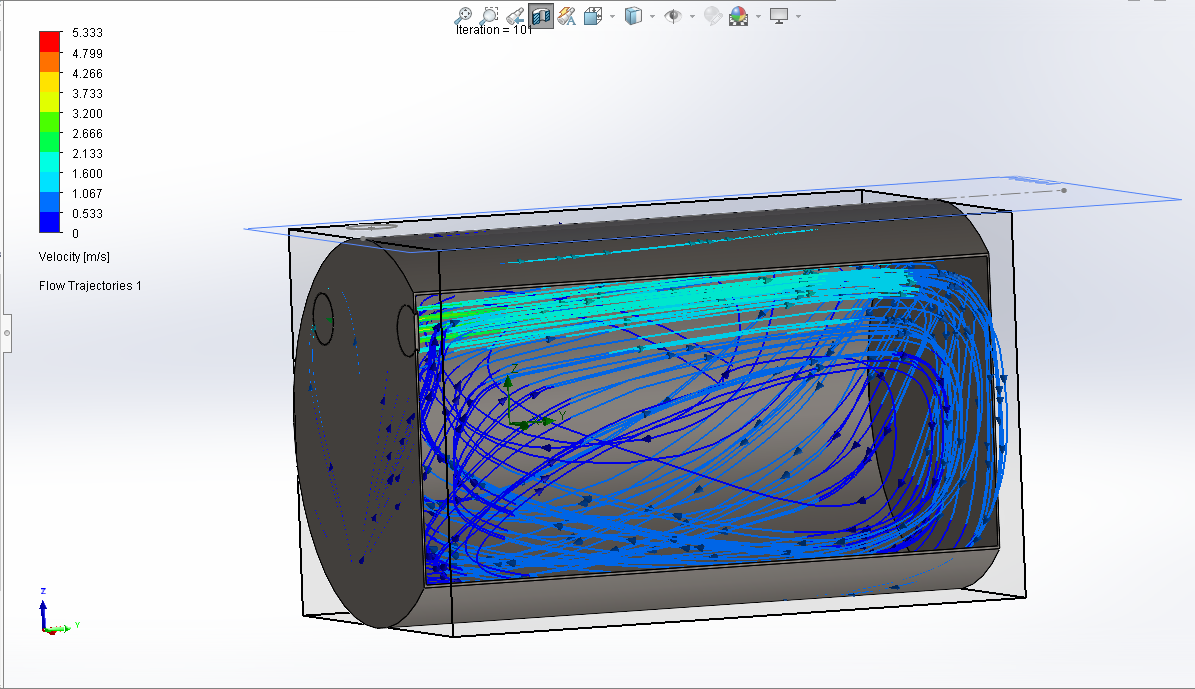
\includegraphics[scale=0.4]{images/Capitulo 4/s5/Contenedor/flow1.png}
            \caption{Configuración de ventiladores en la misma cara lateral}
            \label{fg:ventilador_mcara}
     \end{figure}
    Esta primera configuración \ref{fg:ventilador_mcara},  presenta ambos ventiladores en la misma cara lateral, se observa un recorrido del aire uniforme en el contenedor, sobre todo en la parte inferior del tambo, que es donde se encontrará la mezcla.

    La segunda distribución \ref{fg:ventilador_co},  propuesta, posee los ventiladores en caras laterales opuestas, presentando un comportamiento desordenado y puede notarse que el recorrido no es uniforme, pues existen secciones del contenedor por las que el aire no circula.\newpage
    
     \begin{figure}[h!]
            \centering
            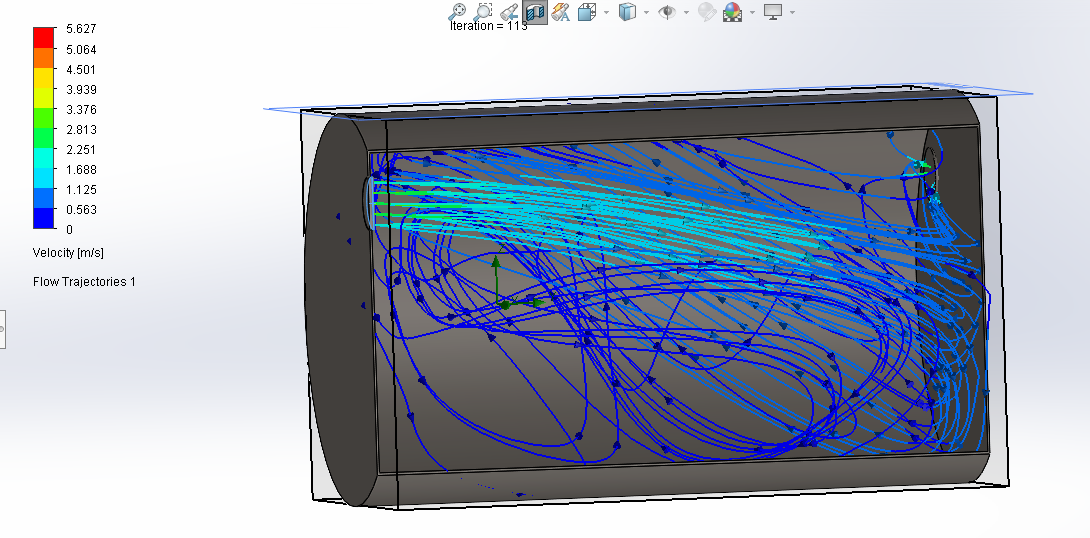
\includegraphics[scale=0.4]{images/Capitulo 4/s5/Contenedor/flow2.png}
            \caption{Configuración de ventiladores en caras laterales opuestas}
            \label{fg:ventilador_co}
     \end{figure}

Para la última configuración se propuso hacer llegar el aire directamente a la mezcla por medio de un tubo introducido por la parte superior del contenedor, llegando unos centimetros arriba del nivel de la mezcla, lo que provocaría la inyección de aire en la parte inferior del tambo. Esta configuración aparente ser muy buena ya que el aire frío por su densidad se localizaría en la parte inferior del contenedor y una vez que el aire se caliente, este ascendería gradualmente y sería expulsado por el otro ventilador, sin embargo se debe tener en cuenta que requerirá de un mayor trabajo de manufactura.

        \begin{figure}[h!]
            \centering
            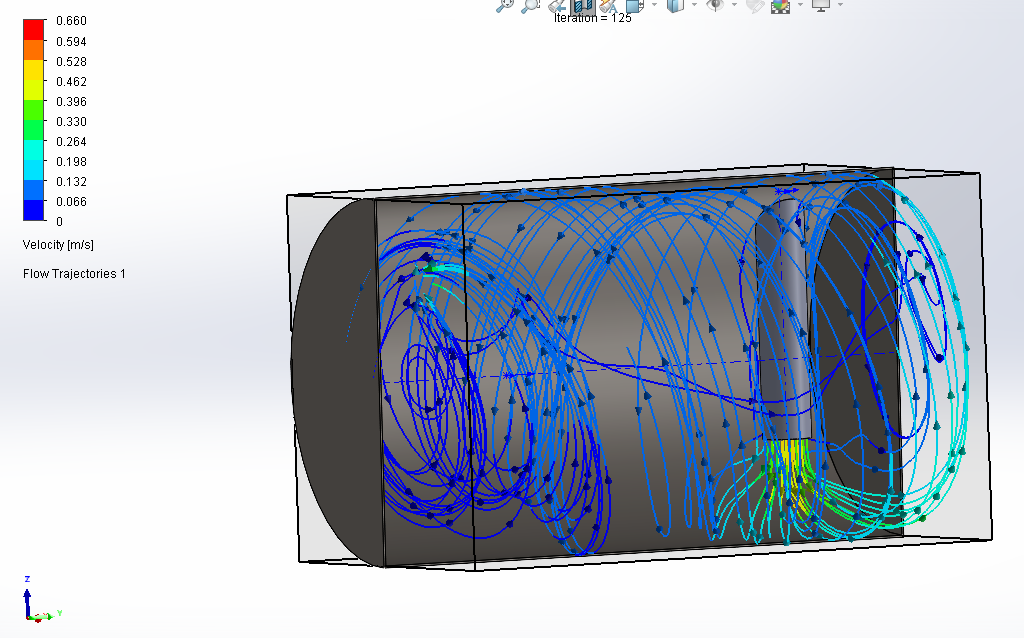
\includegraphics[scale=0.4]{images/Capitulo 4/s5/Contenedor/Flow_Profe_Islas.png}
            \caption{Configuración de ventiladores, aire inyectado directamente en la mezcla }
            \label{fg:ventilador_cilindro}
     \end{figure}


 Como se pudo observar, las distribuciones que mejor se acoplan a lo requerido, serían la primera \ref{fg:ventilador_mcara} y la tercera configuración \ref{fg:ventilador_cilindro}. Y aunque la última propuesta podría tener el mejor comportamiento de las tres, presenta un riesgo en su manufactura pues se requiere la incorporación del cilindro que llevará el aire al interior del contenedor, necesitará de un buen sellado en la parte superior y existe la posibilidad de que el contenedor se dañe quedando inservible, es importante mencionar que el tambo será uno de los componentes más costosos del proyecto por lo que no sería viable para el equipo. Por lo que estaría optando por utilizar la primer configuración, pues la colocación de los ventiladores en la cara lateral del tambo resulta más sencilla  y el riesgo de dañar el contenedor aparenta ser menor.